
% Default to the notebook output style

    


% Inherit from the specified cell style.




    
\documentclass[11pt]{article}

    
    
    \usepackage[T1]{fontenc}
    % Nicer default font (+ math font) than Computer Modern for most use cases
    \usepackage{mathpazo}

    % Basic figure setup, for now with no caption control since it's done
    % automatically by Pandoc (which extracts ![](path) syntax from Markdown).
    \usepackage{graphicx}
    % We will generate all images so they have a width \maxwidth. This means
    % that they will get their normal width if they fit onto the page, but
    % are scaled down if they would overflow the margins.
    \makeatletter
    \def\maxwidth{\ifdim\Gin@nat@width>\linewidth\linewidth
    \else\Gin@nat@width\fi}
    \makeatother
    \let\Oldincludegraphics\includegraphics
    % Set max figure width to be 80% of text width, for now hardcoded.
    \renewcommand{\includegraphics}[1]{\Oldincludegraphics[width=.8\maxwidth]{#1}}
    % Ensure that by default, figures have no caption (until we provide a
    % proper Figure object with a Caption API and a way to capture that
    % in the conversion process - todo).
    \usepackage{caption}
    \DeclareCaptionLabelFormat{nolabel}{}
    \captionsetup{labelformat=nolabel}

    \usepackage{adjustbox} % Used to constrain images to a maximum size 
    \usepackage{xcolor} % Allow colors to be defined
    \usepackage{enumerate} % Needed for markdown enumerations to work
    \usepackage{geometry} % Used to adjust the document margins
    \usepackage{amsmath} % Equations
    \usepackage{amssymb} % Equations
    \usepackage{textcomp} % defines textquotesingle
    % Hack from http://tex.stackexchange.com/a/47451/13684:
    \AtBeginDocument{%
        \def\PYZsq{\textquotesingle}% Upright quotes in Pygmentized code
    }
    \usepackage{upquote} % Upright quotes for verbatim code
    \usepackage{eurosym} % defines \euro
    \usepackage[mathletters]{ucs} % Extended unicode (utf-8) support
    \usepackage[utf8x]{inputenc} % Allow utf-8 characters in the tex document
    \usepackage{fancyvrb} % verbatim replacement that allows latex
    \usepackage{grffile} % extends the file name processing of package graphics 
                         % to support a larger range 
    % The hyperref package gives us a pdf with properly built
    % internal navigation ('pdf bookmarks' for the table of contents,
    % internal cross-reference links, web links for URLs, etc.)
    \usepackage{hyperref}
    \usepackage{longtable} % longtable support required by pandoc >1.10
    \usepackage{booktabs}  % table support for pandoc > 1.12.2
    \usepackage[inline]{enumitem} % IRkernel/repr support (it uses the enumerate* environment)
    \usepackage[normalem]{ulem} % ulem is needed to support strikethroughs (\sout)
                                % normalem makes italics be italics, not underlines
    

    
    
    % Colors for the hyperref package
    \definecolor{urlcolor}{rgb}{0,.145,.698}
    \definecolor{linkcolor}{rgb}{.71,0.21,0.01}
    \definecolor{citecolor}{rgb}{.12,.54,.11}

    % ANSI colors
    \definecolor{ansi-black}{HTML}{3E424D}
    \definecolor{ansi-black-intense}{HTML}{282C36}
    \definecolor{ansi-red}{HTML}{E75C58}
    \definecolor{ansi-red-intense}{HTML}{B22B31}
    \definecolor{ansi-green}{HTML}{00A250}
    \definecolor{ansi-green-intense}{HTML}{007427}
    \definecolor{ansi-yellow}{HTML}{DDB62B}
    \definecolor{ansi-yellow-intense}{HTML}{B27D12}
    \definecolor{ansi-blue}{HTML}{208FFB}
    \definecolor{ansi-blue-intense}{HTML}{0065CA}
    \definecolor{ansi-magenta}{HTML}{D160C4}
    \definecolor{ansi-magenta-intense}{HTML}{A03196}
    \definecolor{ansi-cyan}{HTML}{60C6C8}
    \definecolor{ansi-cyan-intense}{HTML}{258F8F}
    \definecolor{ansi-white}{HTML}{C5C1B4}
    \definecolor{ansi-white-intense}{HTML}{A1A6B2}

    % commands and environments needed by pandoc snippets
    % extracted from the output of `pandoc -s`
    \providecommand{\tightlist}{%
      \setlength{\itemsep}{0pt}\setlength{\parskip}{0pt}}
    \DefineVerbatimEnvironment{Highlighting}{Verbatim}{commandchars=\\\{\}}
    % Add ',fontsize=\small' for more characters per line
    \newenvironment{Shaded}{}{}
    \newcommand{\KeywordTok}[1]{\textcolor[rgb]{0.00,0.44,0.13}{\textbf{{#1}}}}
    \newcommand{\DataTypeTok}[1]{\textcolor[rgb]{0.56,0.13,0.00}{{#1}}}
    \newcommand{\DecValTok}[1]{\textcolor[rgb]{0.25,0.63,0.44}{{#1}}}
    \newcommand{\BaseNTok}[1]{\textcolor[rgb]{0.25,0.63,0.44}{{#1}}}
    \newcommand{\FloatTok}[1]{\textcolor[rgb]{0.25,0.63,0.44}{{#1}}}
    \newcommand{\CharTok}[1]{\textcolor[rgb]{0.25,0.44,0.63}{{#1}}}
    \newcommand{\StringTok}[1]{\textcolor[rgb]{0.25,0.44,0.63}{{#1}}}
    \newcommand{\CommentTok}[1]{\textcolor[rgb]{0.38,0.63,0.69}{\textit{{#1}}}}
    \newcommand{\OtherTok}[1]{\textcolor[rgb]{0.00,0.44,0.13}{{#1}}}
    \newcommand{\AlertTok}[1]{\textcolor[rgb]{1.00,0.00,0.00}{\textbf{{#1}}}}
    \newcommand{\FunctionTok}[1]{\textcolor[rgb]{0.02,0.16,0.49}{{#1}}}
    \newcommand{\RegionMarkerTok}[1]{{#1}}
    \newcommand{\ErrorTok}[1]{\textcolor[rgb]{1.00,0.00,0.00}{\textbf{{#1}}}}
    \newcommand{\NormalTok}[1]{{#1}}
    
    % Additional commands for more recent versions of Pandoc
    \newcommand{\ConstantTok}[1]{\textcolor[rgb]{0.53,0.00,0.00}{{#1}}}
    \newcommand{\SpecialCharTok}[1]{\textcolor[rgb]{0.25,0.44,0.63}{{#1}}}
    \newcommand{\VerbatimStringTok}[1]{\textcolor[rgb]{0.25,0.44,0.63}{{#1}}}
    \newcommand{\SpecialStringTok}[1]{\textcolor[rgb]{0.73,0.40,0.53}{{#1}}}
    \newcommand{\ImportTok}[1]{{#1}}
    \newcommand{\DocumentationTok}[1]{\textcolor[rgb]{0.73,0.13,0.13}{\textit{{#1}}}}
    \newcommand{\AnnotationTok}[1]{\textcolor[rgb]{0.38,0.63,0.69}{\textbf{\textit{{#1}}}}}
    \newcommand{\CommentVarTok}[1]{\textcolor[rgb]{0.38,0.63,0.69}{\textbf{\textit{{#1}}}}}
    \newcommand{\VariableTok}[1]{\textcolor[rgb]{0.10,0.09,0.49}{{#1}}}
    \newcommand{\ControlFlowTok}[1]{\textcolor[rgb]{0.00,0.44,0.13}{\textbf{{#1}}}}
    \newcommand{\OperatorTok}[1]{\textcolor[rgb]{0.40,0.40,0.40}{{#1}}}
    \newcommand{\BuiltInTok}[1]{{#1}}
    \newcommand{\ExtensionTok}[1]{{#1}}
    \newcommand{\PreprocessorTok}[1]{\textcolor[rgb]{0.74,0.48,0.00}{{#1}}}
    \newcommand{\AttributeTok}[1]{\textcolor[rgb]{0.49,0.56,0.16}{{#1}}}
    \newcommand{\InformationTok}[1]{\textcolor[rgb]{0.38,0.63,0.69}{\textbf{\textit{{#1}}}}}
    \newcommand{\WarningTok}[1]{\textcolor[rgb]{0.38,0.63,0.69}{\textbf{\textit{{#1}}}}}
    
    
    % Define a nice break command that doesn't care if a line doesn't already
    % exist.
    \def\br{\hspace*{\fill} \\* }
    % Math Jax compatability definitions
    \def\gt{>}
    \def\lt{<}
    % Document parameters
    \title{workshop-fcf}
    
    
    

    % Pygments definitions
    
\makeatletter
\def\PY@reset{\let\PY@it=\relax \let\PY@bf=\relax%
    \let\PY@ul=\relax \let\PY@tc=\relax%
    \let\PY@bc=\relax \let\PY@ff=\relax}
\def\PY@tok#1{\csname PY@tok@#1\endcsname}
\def\PY@toks#1+{\ifx\relax#1\empty\else%
    \PY@tok{#1}\expandafter\PY@toks\fi}
\def\PY@do#1{\PY@bc{\PY@tc{\PY@ul{%
    \PY@it{\PY@bf{\PY@ff{#1}}}}}}}
\def\PY#1#2{\PY@reset\PY@toks#1+\relax+\PY@do{#2}}

\expandafter\def\csname PY@tok@w\endcsname{\def\PY@tc##1{\textcolor[rgb]{0.73,0.73,0.73}{##1}}}
\expandafter\def\csname PY@tok@c\endcsname{\let\PY@it=\textit\def\PY@tc##1{\textcolor[rgb]{0.25,0.50,0.50}{##1}}}
\expandafter\def\csname PY@tok@cp\endcsname{\def\PY@tc##1{\textcolor[rgb]{0.74,0.48,0.00}{##1}}}
\expandafter\def\csname PY@tok@k\endcsname{\let\PY@bf=\textbf\def\PY@tc##1{\textcolor[rgb]{0.00,0.50,0.00}{##1}}}
\expandafter\def\csname PY@tok@kp\endcsname{\def\PY@tc##1{\textcolor[rgb]{0.00,0.50,0.00}{##1}}}
\expandafter\def\csname PY@tok@kt\endcsname{\def\PY@tc##1{\textcolor[rgb]{0.69,0.00,0.25}{##1}}}
\expandafter\def\csname PY@tok@o\endcsname{\def\PY@tc##1{\textcolor[rgb]{0.40,0.40,0.40}{##1}}}
\expandafter\def\csname PY@tok@ow\endcsname{\let\PY@bf=\textbf\def\PY@tc##1{\textcolor[rgb]{0.67,0.13,1.00}{##1}}}
\expandafter\def\csname PY@tok@nb\endcsname{\def\PY@tc##1{\textcolor[rgb]{0.00,0.50,0.00}{##1}}}
\expandafter\def\csname PY@tok@nf\endcsname{\def\PY@tc##1{\textcolor[rgb]{0.00,0.00,1.00}{##1}}}
\expandafter\def\csname PY@tok@nc\endcsname{\let\PY@bf=\textbf\def\PY@tc##1{\textcolor[rgb]{0.00,0.00,1.00}{##1}}}
\expandafter\def\csname PY@tok@nn\endcsname{\let\PY@bf=\textbf\def\PY@tc##1{\textcolor[rgb]{0.00,0.00,1.00}{##1}}}
\expandafter\def\csname PY@tok@ne\endcsname{\let\PY@bf=\textbf\def\PY@tc##1{\textcolor[rgb]{0.82,0.25,0.23}{##1}}}
\expandafter\def\csname PY@tok@nv\endcsname{\def\PY@tc##1{\textcolor[rgb]{0.10,0.09,0.49}{##1}}}
\expandafter\def\csname PY@tok@no\endcsname{\def\PY@tc##1{\textcolor[rgb]{0.53,0.00,0.00}{##1}}}
\expandafter\def\csname PY@tok@nl\endcsname{\def\PY@tc##1{\textcolor[rgb]{0.63,0.63,0.00}{##1}}}
\expandafter\def\csname PY@tok@ni\endcsname{\let\PY@bf=\textbf\def\PY@tc##1{\textcolor[rgb]{0.60,0.60,0.60}{##1}}}
\expandafter\def\csname PY@tok@na\endcsname{\def\PY@tc##1{\textcolor[rgb]{0.49,0.56,0.16}{##1}}}
\expandafter\def\csname PY@tok@nt\endcsname{\let\PY@bf=\textbf\def\PY@tc##1{\textcolor[rgb]{0.00,0.50,0.00}{##1}}}
\expandafter\def\csname PY@tok@nd\endcsname{\def\PY@tc##1{\textcolor[rgb]{0.67,0.13,1.00}{##1}}}
\expandafter\def\csname PY@tok@s\endcsname{\def\PY@tc##1{\textcolor[rgb]{0.73,0.13,0.13}{##1}}}
\expandafter\def\csname PY@tok@sd\endcsname{\let\PY@it=\textit\def\PY@tc##1{\textcolor[rgb]{0.73,0.13,0.13}{##1}}}
\expandafter\def\csname PY@tok@si\endcsname{\let\PY@bf=\textbf\def\PY@tc##1{\textcolor[rgb]{0.73,0.40,0.53}{##1}}}
\expandafter\def\csname PY@tok@se\endcsname{\let\PY@bf=\textbf\def\PY@tc##1{\textcolor[rgb]{0.73,0.40,0.13}{##1}}}
\expandafter\def\csname PY@tok@sr\endcsname{\def\PY@tc##1{\textcolor[rgb]{0.73,0.40,0.53}{##1}}}
\expandafter\def\csname PY@tok@ss\endcsname{\def\PY@tc##1{\textcolor[rgb]{0.10,0.09,0.49}{##1}}}
\expandafter\def\csname PY@tok@sx\endcsname{\def\PY@tc##1{\textcolor[rgb]{0.00,0.50,0.00}{##1}}}
\expandafter\def\csname PY@tok@m\endcsname{\def\PY@tc##1{\textcolor[rgb]{0.40,0.40,0.40}{##1}}}
\expandafter\def\csname PY@tok@gh\endcsname{\let\PY@bf=\textbf\def\PY@tc##1{\textcolor[rgb]{0.00,0.00,0.50}{##1}}}
\expandafter\def\csname PY@tok@gu\endcsname{\let\PY@bf=\textbf\def\PY@tc##1{\textcolor[rgb]{0.50,0.00,0.50}{##1}}}
\expandafter\def\csname PY@tok@gd\endcsname{\def\PY@tc##1{\textcolor[rgb]{0.63,0.00,0.00}{##1}}}
\expandafter\def\csname PY@tok@gi\endcsname{\def\PY@tc##1{\textcolor[rgb]{0.00,0.63,0.00}{##1}}}
\expandafter\def\csname PY@tok@gr\endcsname{\def\PY@tc##1{\textcolor[rgb]{1.00,0.00,0.00}{##1}}}
\expandafter\def\csname PY@tok@ge\endcsname{\let\PY@it=\textit}
\expandafter\def\csname PY@tok@gs\endcsname{\let\PY@bf=\textbf}
\expandafter\def\csname PY@tok@gp\endcsname{\let\PY@bf=\textbf\def\PY@tc##1{\textcolor[rgb]{0.00,0.00,0.50}{##1}}}
\expandafter\def\csname PY@tok@go\endcsname{\def\PY@tc##1{\textcolor[rgb]{0.53,0.53,0.53}{##1}}}
\expandafter\def\csname PY@tok@gt\endcsname{\def\PY@tc##1{\textcolor[rgb]{0.00,0.27,0.87}{##1}}}
\expandafter\def\csname PY@tok@err\endcsname{\def\PY@bc##1{\setlength{\fboxsep}{0pt}\fcolorbox[rgb]{1.00,0.00,0.00}{1,1,1}{\strut ##1}}}
\expandafter\def\csname PY@tok@kc\endcsname{\let\PY@bf=\textbf\def\PY@tc##1{\textcolor[rgb]{0.00,0.50,0.00}{##1}}}
\expandafter\def\csname PY@tok@kd\endcsname{\let\PY@bf=\textbf\def\PY@tc##1{\textcolor[rgb]{0.00,0.50,0.00}{##1}}}
\expandafter\def\csname PY@tok@kn\endcsname{\let\PY@bf=\textbf\def\PY@tc##1{\textcolor[rgb]{0.00,0.50,0.00}{##1}}}
\expandafter\def\csname PY@tok@kr\endcsname{\let\PY@bf=\textbf\def\PY@tc##1{\textcolor[rgb]{0.00,0.50,0.00}{##1}}}
\expandafter\def\csname PY@tok@bp\endcsname{\def\PY@tc##1{\textcolor[rgb]{0.00,0.50,0.00}{##1}}}
\expandafter\def\csname PY@tok@fm\endcsname{\def\PY@tc##1{\textcolor[rgb]{0.00,0.00,1.00}{##1}}}
\expandafter\def\csname PY@tok@vc\endcsname{\def\PY@tc##1{\textcolor[rgb]{0.10,0.09,0.49}{##1}}}
\expandafter\def\csname PY@tok@vg\endcsname{\def\PY@tc##1{\textcolor[rgb]{0.10,0.09,0.49}{##1}}}
\expandafter\def\csname PY@tok@vi\endcsname{\def\PY@tc##1{\textcolor[rgb]{0.10,0.09,0.49}{##1}}}
\expandafter\def\csname PY@tok@vm\endcsname{\def\PY@tc##1{\textcolor[rgb]{0.10,0.09,0.49}{##1}}}
\expandafter\def\csname PY@tok@sa\endcsname{\def\PY@tc##1{\textcolor[rgb]{0.73,0.13,0.13}{##1}}}
\expandafter\def\csname PY@tok@sb\endcsname{\def\PY@tc##1{\textcolor[rgb]{0.73,0.13,0.13}{##1}}}
\expandafter\def\csname PY@tok@sc\endcsname{\def\PY@tc##1{\textcolor[rgb]{0.73,0.13,0.13}{##1}}}
\expandafter\def\csname PY@tok@dl\endcsname{\def\PY@tc##1{\textcolor[rgb]{0.73,0.13,0.13}{##1}}}
\expandafter\def\csname PY@tok@s2\endcsname{\def\PY@tc##1{\textcolor[rgb]{0.73,0.13,0.13}{##1}}}
\expandafter\def\csname PY@tok@sh\endcsname{\def\PY@tc##1{\textcolor[rgb]{0.73,0.13,0.13}{##1}}}
\expandafter\def\csname PY@tok@s1\endcsname{\def\PY@tc##1{\textcolor[rgb]{0.73,0.13,0.13}{##1}}}
\expandafter\def\csname PY@tok@mb\endcsname{\def\PY@tc##1{\textcolor[rgb]{0.40,0.40,0.40}{##1}}}
\expandafter\def\csname PY@tok@mf\endcsname{\def\PY@tc##1{\textcolor[rgb]{0.40,0.40,0.40}{##1}}}
\expandafter\def\csname PY@tok@mh\endcsname{\def\PY@tc##1{\textcolor[rgb]{0.40,0.40,0.40}{##1}}}
\expandafter\def\csname PY@tok@mi\endcsname{\def\PY@tc##1{\textcolor[rgb]{0.40,0.40,0.40}{##1}}}
\expandafter\def\csname PY@tok@il\endcsname{\def\PY@tc##1{\textcolor[rgb]{0.40,0.40,0.40}{##1}}}
\expandafter\def\csname PY@tok@mo\endcsname{\def\PY@tc##1{\textcolor[rgb]{0.40,0.40,0.40}{##1}}}
\expandafter\def\csname PY@tok@ch\endcsname{\let\PY@it=\textit\def\PY@tc##1{\textcolor[rgb]{0.25,0.50,0.50}{##1}}}
\expandafter\def\csname PY@tok@cm\endcsname{\let\PY@it=\textit\def\PY@tc##1{\textcolor[rgb]{0.25,0.50,0.50}{##1}}}
\expandafter\def\csname PY@tok@cpf\endcsname{\let\PY@it=\textit\def\PY@tc##1{\textcolor[rgb]{0.25,0.50,0.50}{##1}}}
\expandafter\def\csname PY@tok@c1\endcsname{\let\PY@it=\textit\def\PY@tc##1{\textcolor[rgb]{0.25,0.50,0.50}{##1}}}
\expandafter\def\csname PY@tok@cs\endcsname{\let\PY@it=\textit\def\PY@tc##1{\textcolor[rgb]{0.25,0.50,0.50}{##1}}}

\def\PYZbs{\char`\\}
\def\PYZus{\char`\_}
\def\PYZob{\char`\{}
\def\PYZcb{\char`\}}
\def\PYZca{\char`\^}
\def\PYZam{\char`\&}
\def\PYZlt{\char`\<}
\def\PYZgt{\char`\>}
\def\PYZsh{\char`\#}
\def\PYZpc{\char`\%}
\def\PYZdl{\char`\$}
\def\PYZhy{\char`\-}
\def\PYZsq{\char`\'}
\def\PYZdq{\char`\"}
\def\PYZti{\char`\~}
% for compatibility with earlier versions
\def\PYZat{@}
\def\PYZlb{[}
\def\PYZrb{]}
\makeatother


    % Exact colors from NB
    \definecolor{incolor}{rgb}{0.0, 0.0, 0.5}
    \definecolor{outcolor}{rgb}{0.545, 0.0, 0.0}



    
    % Prevent overflowing lines due to hard-to-break entities
    \sloppy 
    % Setup hyperref package
    \hypersetup{
      breaklinks=true,  % so long urls are correctly broken across lines
      colorlinks=true,
      urlcolor=urlcolor,
      linkcolor=linkcolor,
      citecolor=citecolor,
      }
    % Slightly bigger margins than the latex defaults
    
    \geometry{verbose,tmargin=1in,bmargin=1in,lmargin=1in,rmargin=1in}
    
    

    \begin{document}
    
    
    \maketitle
    
    

    
    \section{\texorpdfstring{Cálculo científico con Jupyter -
\emph{"Talleres que
molan"}}{Cálculo científico con Jupyter - "Talleres que molan"}}\label{cuxe1lculo-cientuxedfico-con-jupyter---talleres-que-molan}

    

    \textbf{Ponente:} \href{https://albertopastormr.me/}{Alberto Pastor
Moreno} - {[}@albertopastormr{]}(https://twitter.com/albertopastormr)

\textbf{Organizado por:}

\begin{itemize}
\item
  \href{https://www.ucm.es/oficina-de-software-libre/}{Oficina de
  Software Libre de la Universidad Complutense de Madrid}
  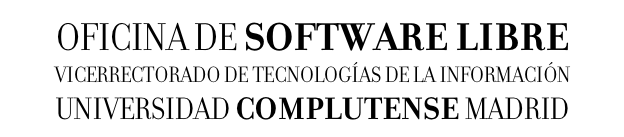
\includegraphics{otea.png}
\item
  \href{https://scidataucm.org/}{SciData} 
\item
  \href{https://fisicas.ucm.es/}{Facultad de Ciencias Físicas} 
\end{itemize}

    \subsection{Project Jupyter}\label{project-jupyter}

    \begin{figure}
\centering

\includegraphics{jupyter-logo2.png}
\caption{}
\end{figure}

    \href{https://jupyter.org/about}{Project Jupyter} es una organización
sin ánimo de lucro que desarrolla y mantiene software libre con
\href{https://opensource.org/licenses/BSD-3-Clause}{licencia BSD}. Nació
en 2014 desde el proyecto ya previamente existente
\href{https://ipython.org/}{IPython} (hablaremos más adelante de ello).
Prácticamente toda su operativa se resume en desarrollar y construir
sobre el entorno Notebook, del que hablaremos más adelante. Por ello,
son responsables del desarrollo de proyectos como
\href{https://mybinder.org/}{Binder},
\href{https://nbviewer.jupyter.org/}{NBViewer} y
\href{https://jupyter.org/hub}{JupyterHub}; todos se integran con
arquitectura Notebook. Project Jupyter recibe el soporte de
\href{https://numfocus.org/}{NumFocus}, organización que vela por el
desarrollo de herramientas científicas open-source con el objetivo de
conseguir una ciencia amplia y abierta. La comunidad de Project Jupyter
es realmente extensa, tanto es así que organizan colaborativamente
\href{https://t.co/NjJypi80sj}{JupyterCon}. Si quieres participar en la
comunidad, no olvides leer
\href{https://github.com/jupyter/governance/blob/master/conduct/code_of_conduct.md}{su
código de conducta}.

Puedes encontrar todos los proyectos de Project Jupyter en los
repositorios almacenados bajo su organización en GitHub
\href{https://github.com/jupyter}{aquí}.

La documentación oficial de todo el software desarrollado por Project
Jupyter la puedes encontrar
\href{https://jupyter.org/documentation}{aquí}.

    \subsection{Jupyter Notebook}\label{jupyter-notebook}

    Jupyter Notebook es un formato de documento abierto basado en JSON. Los
documentos Jupyter Notebook contienen código ejecutable, texto rico en
formateado con Markdown, ecuaciones con LaTeX y visualizaciones sin
límites. Jupyter Notebook es un proyecto de Project Jupyter cuyo
objetivo es facilitar la edición de textos científicos, agregándoles una
nueva dimensión de interacción en la lectura permitiendo ejecutar el
código citado en el documento. Jupyter Notebook es utilizado a diario
por entidades tan relevantes en el la industria tecnológica como Google,
Microsoft e IBM y por investigadores de instituciones de la talla de
Berkeley o NASA.

    \begin{figure}
\centering
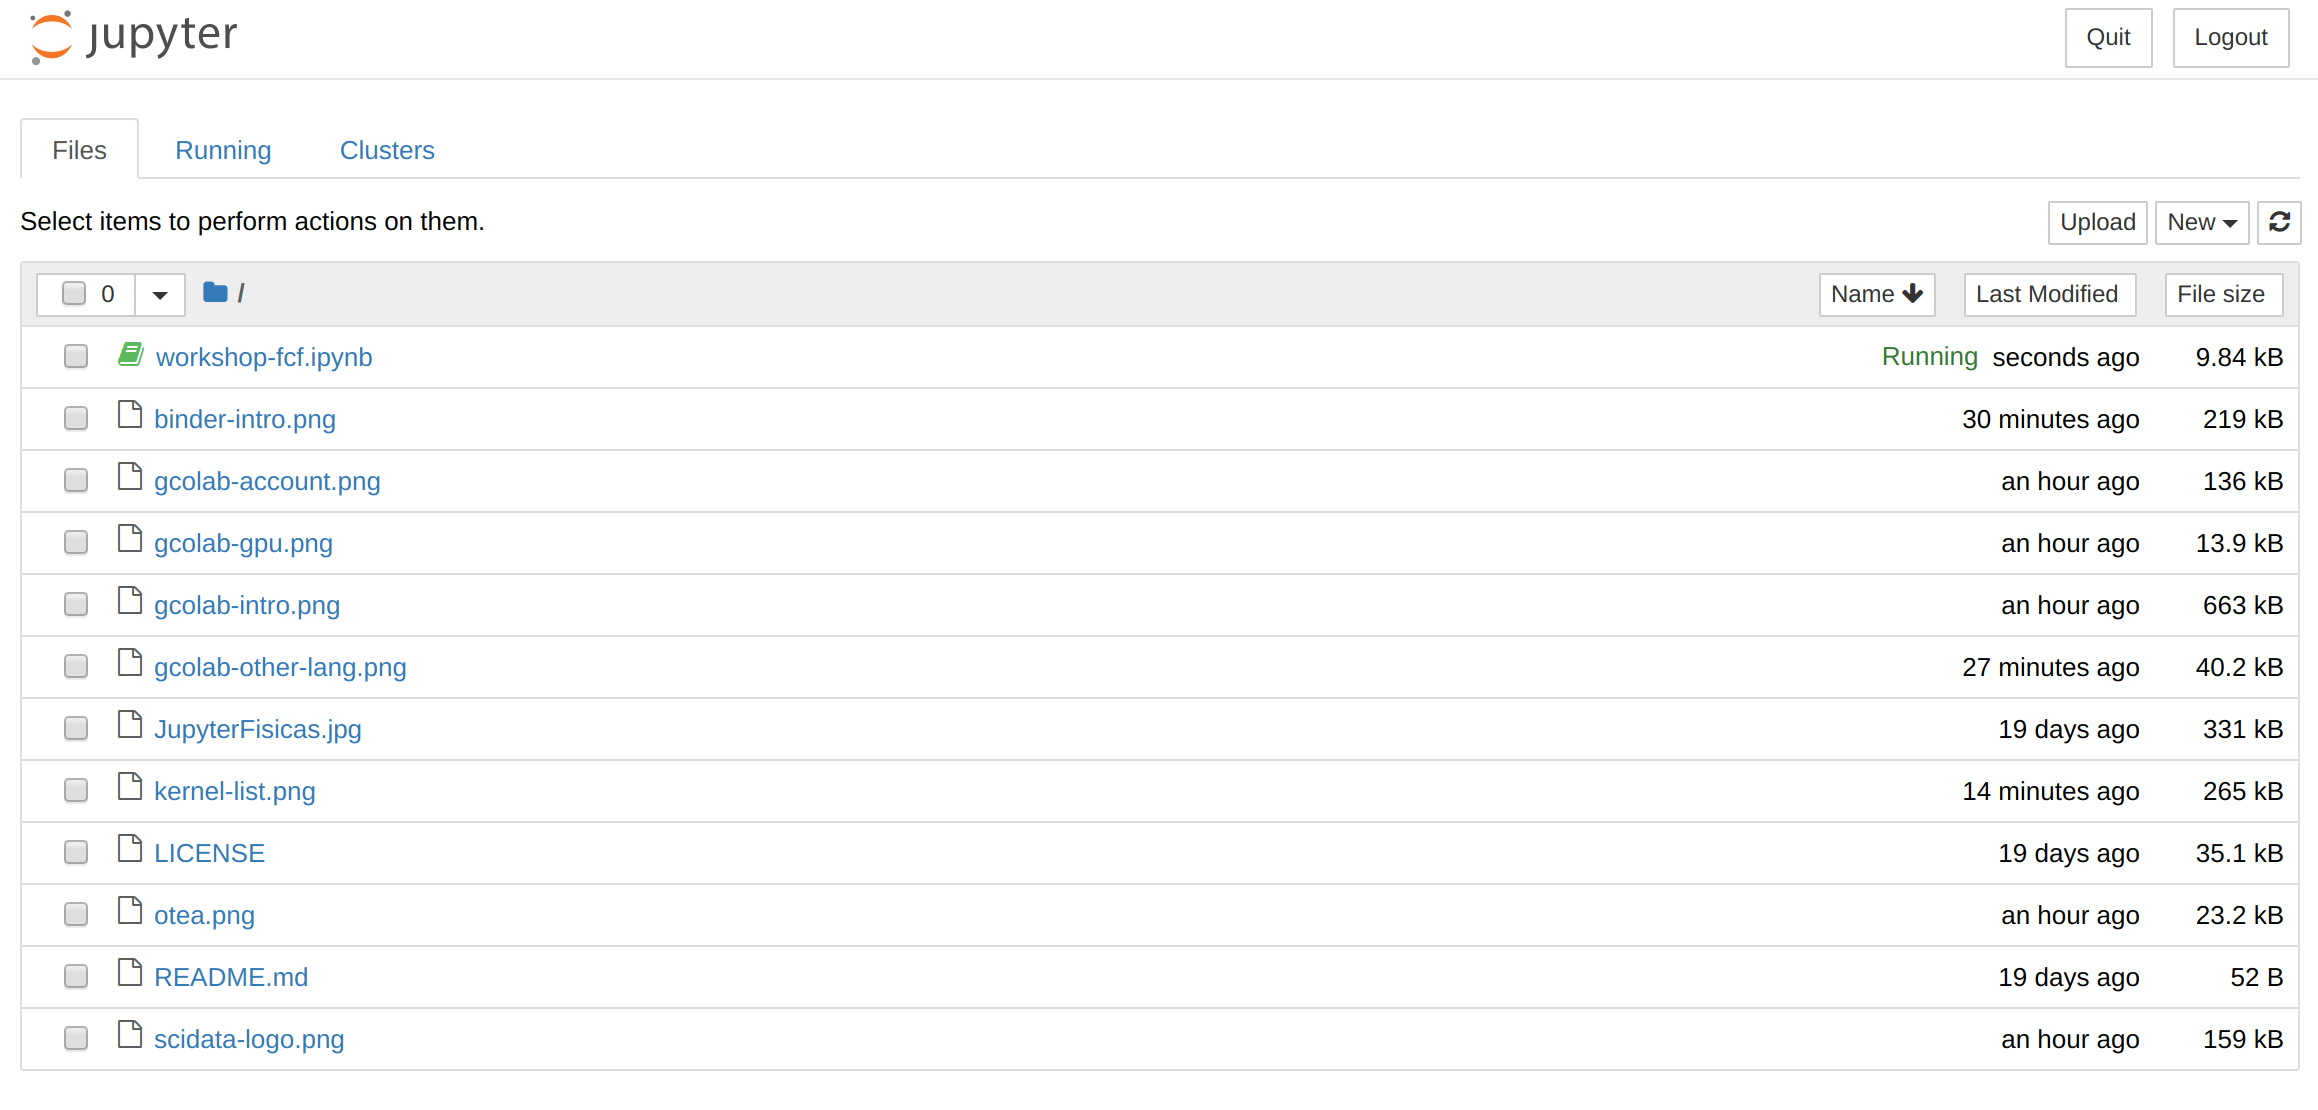
\includegraphics{jupyter-ui.png}
\caption{}
\end{figure}

    A continuación veremos los pilares de Jupyter Notebook que nos ayudarán
a entender levemente cómo funciona internamente.

    \subsubsection{Celdas}\label{celdas}

    Los documentos Jupyter Notebook se componen de una secuencia de celdas
que contienen código o texto. Jupyter Notebook comtempla dos tipos
diferentes de celdas: - Celdas de código: cuando son ejecutadas se
procesan las intrucciones alojadas en la celda. Si las instrucciones
ejecutadas tuvieran salida o alguna instrucción que escribe en pantalla
como \texttt{print()}, se escribiría el resultado a continuación de la
celda. - Celdas Markdown: cuando son ejecutadas se maqueta el texto
alojado en la celda.

Hasta ahora, no has visto ninguna celda de código, todas las celdas del
documento hasta este instante, incluidas las que muestran imágenes y
enlaces, son celdas Markdown. Por lo tanto, este texto, se encuentra en
una celda Markdown. Volveremos con ello más adelante.

    La siguiente celda es una celda de código que ejecuta una suma
escribiendo en pantalla el resultado:

    \begin{Verbatim}[commandchars=\\\{\}]
{\color{incolor}In [{\color{incolor}1}]:} \PY{l+m+mi}{2} \PY{o}{+} \PY{l+m+mi}{2}
\end{Verbatim}


\begin{Verbatim}[commandchars=\\\{\}]
{\color{outcolor}Out[{\color{outcolor}1}]:} 4
\end{Verbatim}
            
    Las celdas de código pueden contener una o muchas instrucciones;
simplemente escribe código como lo harías en un IDE cualquiera pero
dividiendo el código en secciones (celdas) lógicamente separadas. De
esta forma, tendrás un documento limpio y fácilmente mantenible,
pudiendo probar pequeñas porciones de código con variables declaradas en
celdas anteriores.

    A continuación se muestra una celda de código que realiza algunas
instrucciones Python algo más complejas que el ejemplo anterior:

    \begin{Verbatim}[commandchars=\\\{\}]
{\color{incolor}In [{\color{incolor}2}]:} \PY{k}{for} \PY{n}{i} \PY{o+ow}{in} \PY{n+nb}{range}\PY{p}{(}\PY{l+m+mi}{0}\PY{p}{,}\PY{l+m+mi}{10}\PY{p}{)}\PY{p}{:}
            \PY{n+nb}{print}\PY{p}{(}\PY{l+s+s1}{\PYZsq{}}\PY{l+s+s1}{Vuelta del bucle numero }\PY{l+s+s1}{\PYZsq{}}\PY{p}{,} \PY{n}{i}\PY{p}{)}
\end{Verbatim}


    \begin{Verbatim}[commandchars=\\\{\}]
Vuelta del bucle numero  0
Vuelta del bucle numero  1
Vuelta del bucle numero  2
Vuelta del bucle numero  3
Vuelta del bucle numero  4
Vuelta del bucle numero  5
Vuelta del bucle numero  6
Vuelta del bucle numero  7
Vuelta del bucle numero  8
Vuelta del bucle numero  9

    \end{Verbatim}

    Como has podido comprobar, la salida de la ejecución de una celda de
código puede concatenar varias instrucciones de impresión.

    \begin{Verbatim}[commandchars=\\\{\}]
{\color{incolor}In [{\color{incolor}3}]:} \PY{n}{a} \PY{o}{=} \PY{l+m+mi}{2}
\end{Verbatim}


    La celda superior no ha mostrado nada. Esto se debe a que su instrucción
ha sido una asignación a una variable \texttt{a}, la cual, tras la
ejecución de la celda, pasa a estar disponible en todo el presente
documento Notebook con su correspondiente valor asignado.

Todas las variables utilizadas en el documento Notebook pasan a una
\emph{bolsa} de variables activas que pueden ser utilizadas en cualquier
celda de código.

    \begin{Verbatim}[commandchars=\\\{\}]
{\color{incolor}In [{\color{incolor}4}]:} \PY{n+nb}{print}\PY{p}{(}\PY{n}{a}\PY{p}{)}
\end{Verbatim}


    \begin{Verbatim}[commandchars=\\\{\}]
2

    \end{Verbatim}

    También podemos modificar el valor de \texttt{a} en cualquier celda

    \begin{Verbatim}[commandchars=\\\{\}]
{\color{incolor}In [{\color{incolor}5}]:} \PY{n}{a} \PY{o}{=} \PY{l+m+mi}{3}
\end{Verbatim}


    \begin{Verbatim}[commandchars=\\\{\}]
{\color{incolor}In [{\color{incolor}6}]:} \PY{n+nb}{print}\PY{p}{(}\PY{n}{a}\PY{p}{)}
\end{Verbatim}


    \begin{Verbatim}[commandchars=\\\{\}]
3

    \end{Verbatim}

    Ahora, todas las celdas del documento conocen a la variable \texttt{a}
con el valor 3. Por lo tanto, podemos utilizarla considerando esto:

    \begin{Verbatim}[commandchars=\\\{\}]
{\color{incolor}In [{\color{incolor}7}]:} \PY{l+m+mi}{2} \PY{o}{+} \PY{n}{a} 
\end{Verbatim}


\begin{Verbatim}[commandchars=\\\{\}]
{\color{outcolor}Out[{\color{outcolor}7}]:} 5
\end{Verbatim}
            
    Si aplicas estos conceptos al desarrollo de tu código, podrás diseñar
cualquier análisis o experimento científico construyendo celdas como
hemos hecho hasta ahora.

    \subsubsection{Kernel}\label{kernel}

    Un kernel es un motor computacional sobre el cual se ejecuta cada una de
las celdas de código del documento; cada documento Notebook tiene
asignado un kernel. El kernel de un documento Notebook persiste en el
tiempo y las ejecuciones de celdas, por lo tanto, si declaras una
variable en la ejecución de una instrucción, esa variable será accesible
en cualquier posible futura ejecución de otra instrucción (o la misma
instrucción). Lo mismo ocurre con ejecuciones de instrucciones
\texttt{import}; aquello que haya sido importado una vez, estará
disponible en todas las celdas.

    \begin{figure}
\centering
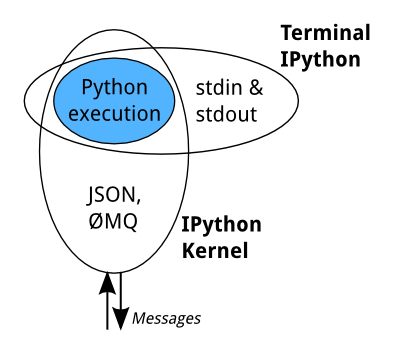
\includegraphics{kernel-pipeline.png}
\caption{}
\end{figure}

    \subsection{Markdown}\label{markdown}

    Markdown es un lenguaje de marcado ligero creado en el 2004 que permite
formatear textos con apenas algunos comandos simples y sencillos de
aprender y aplicar. A pesar de haber recibido diferentes versiones (por
ejemplo, GitHub usa su propia versión para interpretar ficheros Markdown
alojados en sus repositorios), Markdown ha sido estandarizado en
múltiples herramientas como Jupyter. Markdown realiza de puente con
código HTML exponiendo una usabilidad mucho más amigable. Es por ello
por lo cual en celdas Markdown también se puede ejecutar código HTML.

La siguiente imagen resume la mayoría de comandos necesarios para
formatear prácticamente cualquier texto.

    \begin{figure}
\centering
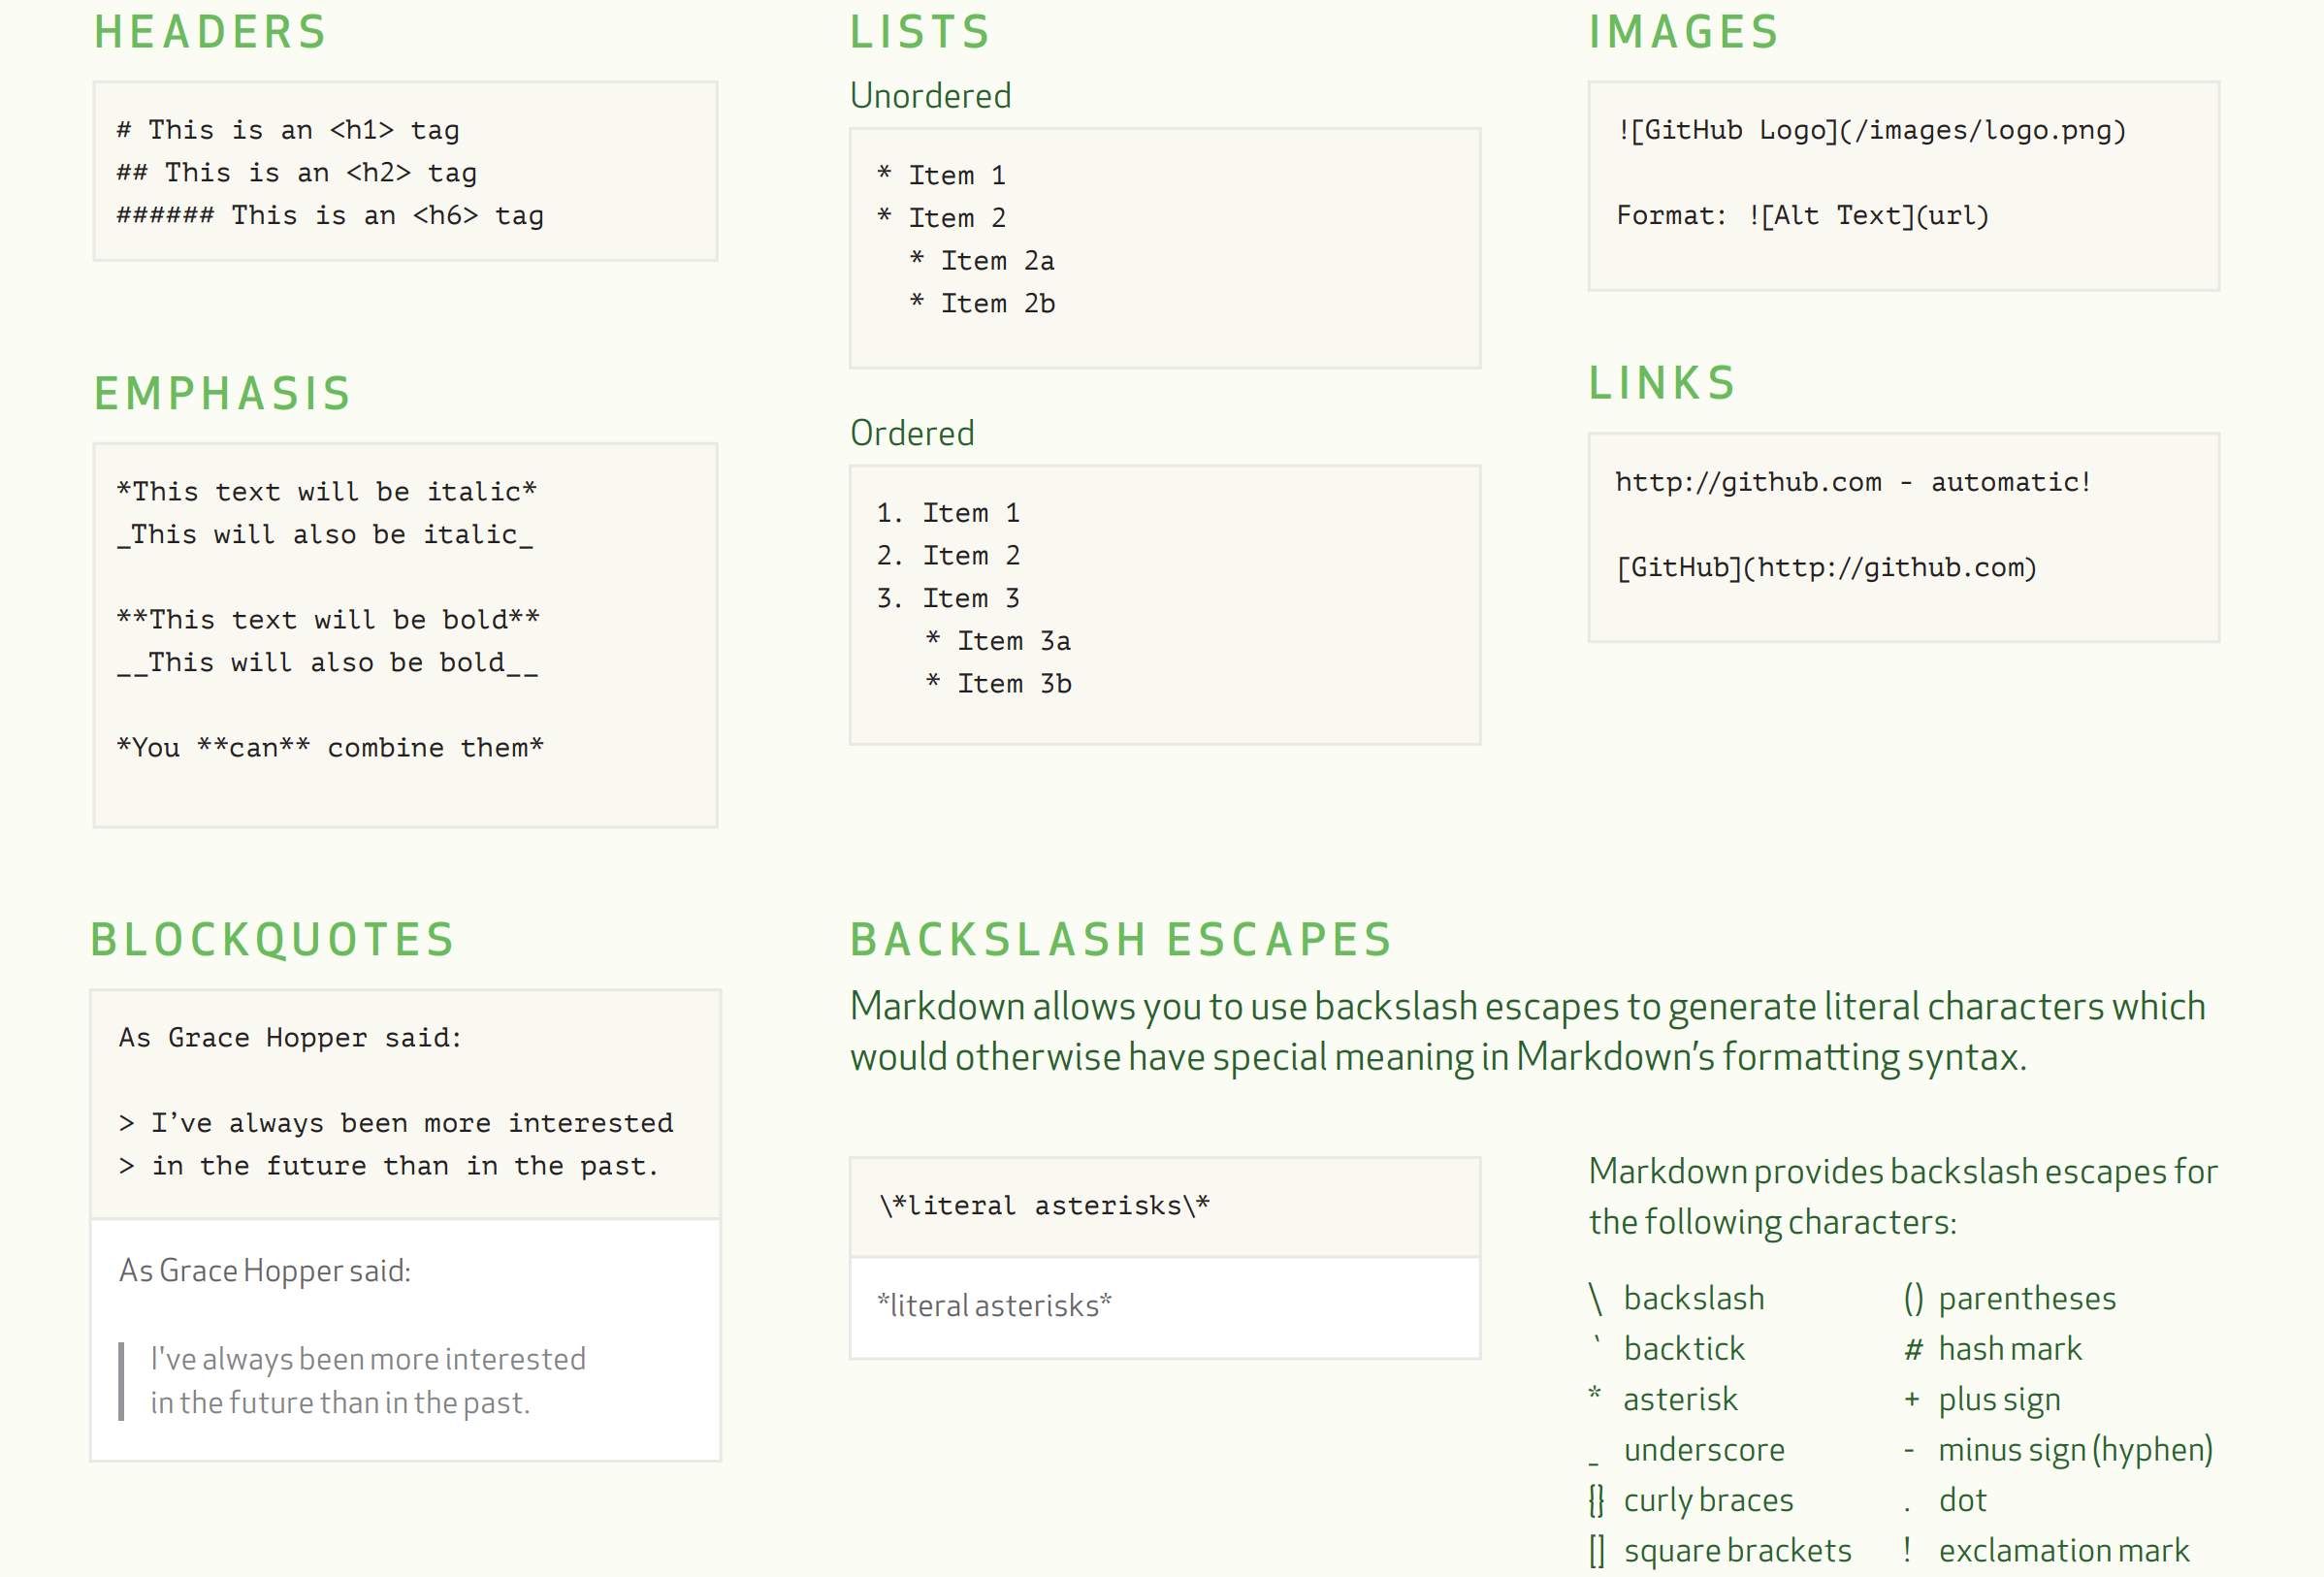
\includegraphics{markdown-cheatsheet.png}
\caption{}
\end{figure}

    Al ejecutar una celda Markdown veremos cómo traduce el sistema nuestro
texto escrito.

Markdown permite utilizar sintaxis más avanzada que la expuesta en la
imagen, como por ejemplo la sintaxis necesaria para crear una tabla.
Para ello, recomiendo visitar
\href{https://github.com/adam-p/markdown-here/wiki/Markdown-Cheatsheet}{este
enlace}

    Markdown, además, permite utilizar el modo matemático de LaTeX, lo cual
da lugar a un sinfín de posibilidades en la redacción de nuestros
documentos con Jupyter:

\[ x = \sum_{i=0}^{N}{y^2} \]

    \subsection{IPython}\label{ipython}

    \href{}{IPython} es una herramienta de computación interactiva integrada
bajo el ámbito de Project Jupyter. Los documentos Notebook originalmente
eran una característica de IPython hasta 2014, cuando Jupyter Notebook
se formó utilizando IPython como kernel. IPython proporciona una
\emph{shell} interactiva con características como resaltado de líneas
que no ofrece la \emph{shell} predeterminada de Python.

    \begin{figure}
\centering
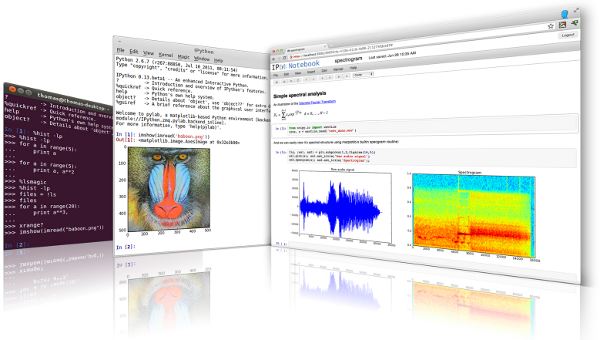
\includegraphics{ipython.png}
\caption{}
\end{figure}

    \subsection{Otros kernels}\label{otros-kernels}

    Dado que Jupyter es software libre, la comunidad de usuarios ha
desarrollado múltiples kernels para bastantes lenguajes no nativos en la
herramienta, como R, Scala, Matlab y Octave. Puedes encontrar un enlace
a todos los kernels disponibles
\href{https://github.com/jupyter/jupyter/wiki/Jupyter-kernels}{aquí}.

    \begin{figure}
\centering
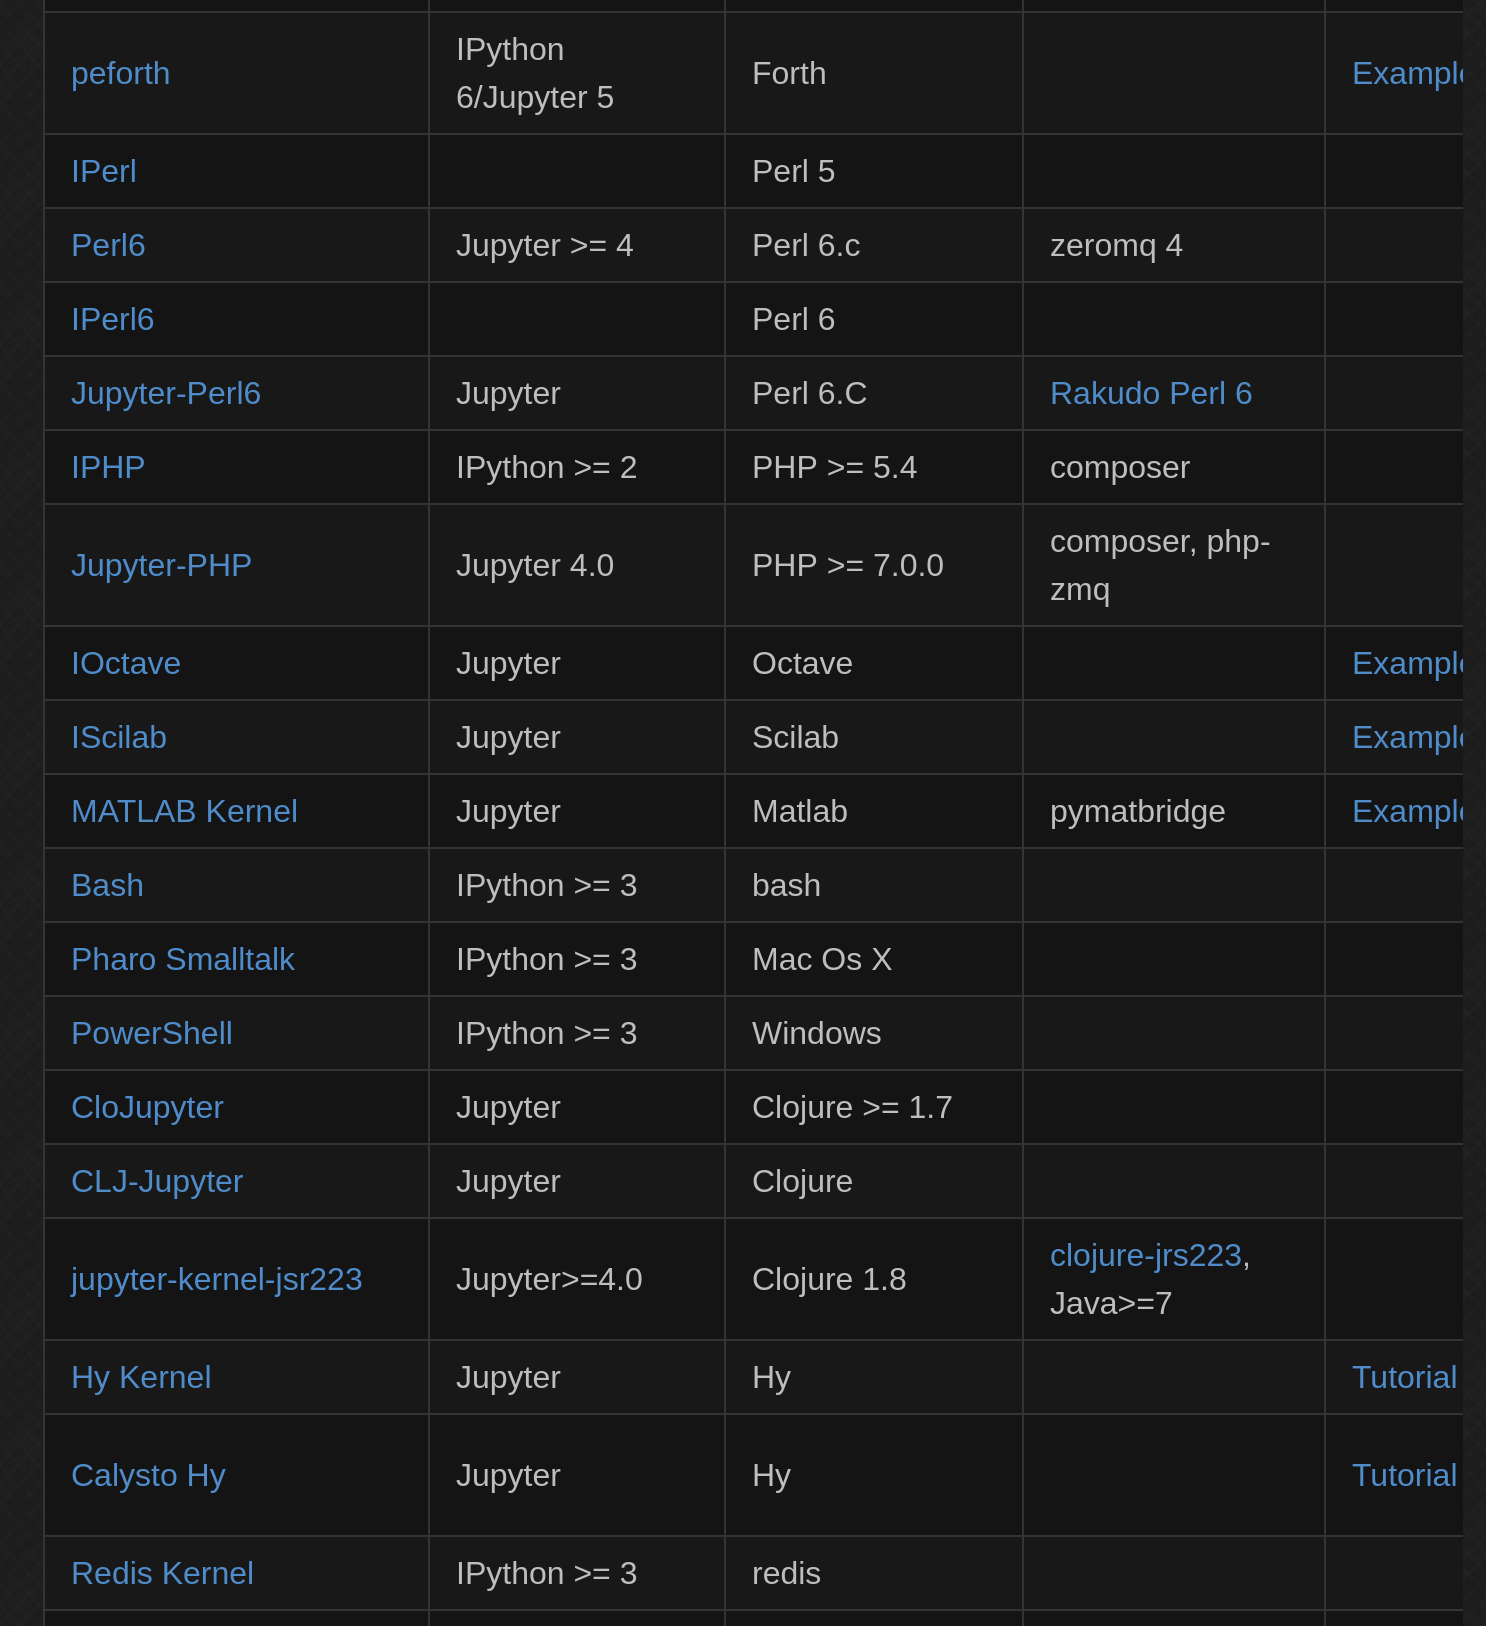
\includegraphics{kernel-list.png}
\caption{}
\end{figure}

    Si quieres desarrollar en un lenguaje que no sea Python, no hay ningún
problema, ya que eligiendo el kernel que necesites con unos pocos pasos
podrás crear y editar documentos Notebook en otros lenguajes.

    \subsection{Exportar Jupyter Notebook en
PDF}\label{exportar-jupyter-notebook-en-pdf}

    Una vez has realizado todos tus experimentos y análisis en tu documento
Notebook, te gustaría poder enseñarle a tus compañeros o profesores lo
que has hecho en tu Notebook, mostrando tu documentación y código. Para
ello, puedes exportar cualquier documento Notebook en un documento PDF,
un formato más aceptado universalmente, desde el propio Jupyter.

    \begin{figure}
\centering
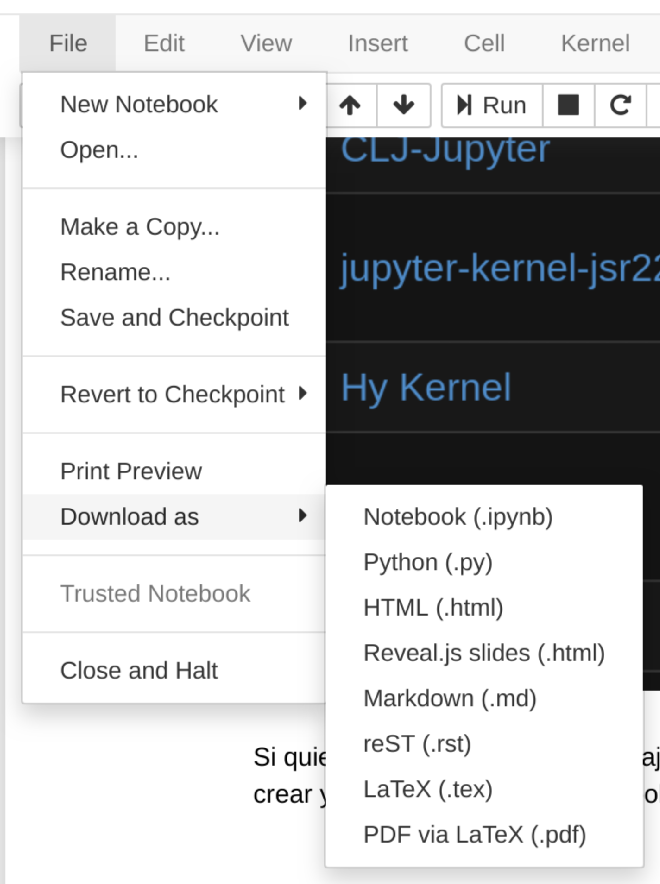
\includegraphics{export-pdf.png}
\caption{}
\end{figure}

    \subsection{Binder}\label{binder}

    \href{https://mybinder.org/}{Binder}, herramienta desarrollada y
mantenida por Project Jupyter, permite abrir y compartir un fichero
Notebook con un entorno ejecutable sin preocuparse por las dependencias
necesarias (librerías) desde un repositorio alojado en GitHub. Binder no
requiere tener Jupyter Notebook instalado; simplemente accede a un
Notebook hosteado con Binder desde un navegador web y al instante podrás
modificar el contenido del Notebook y ejecutar cualquier celda de
código.

    \begin{figure}
\centering
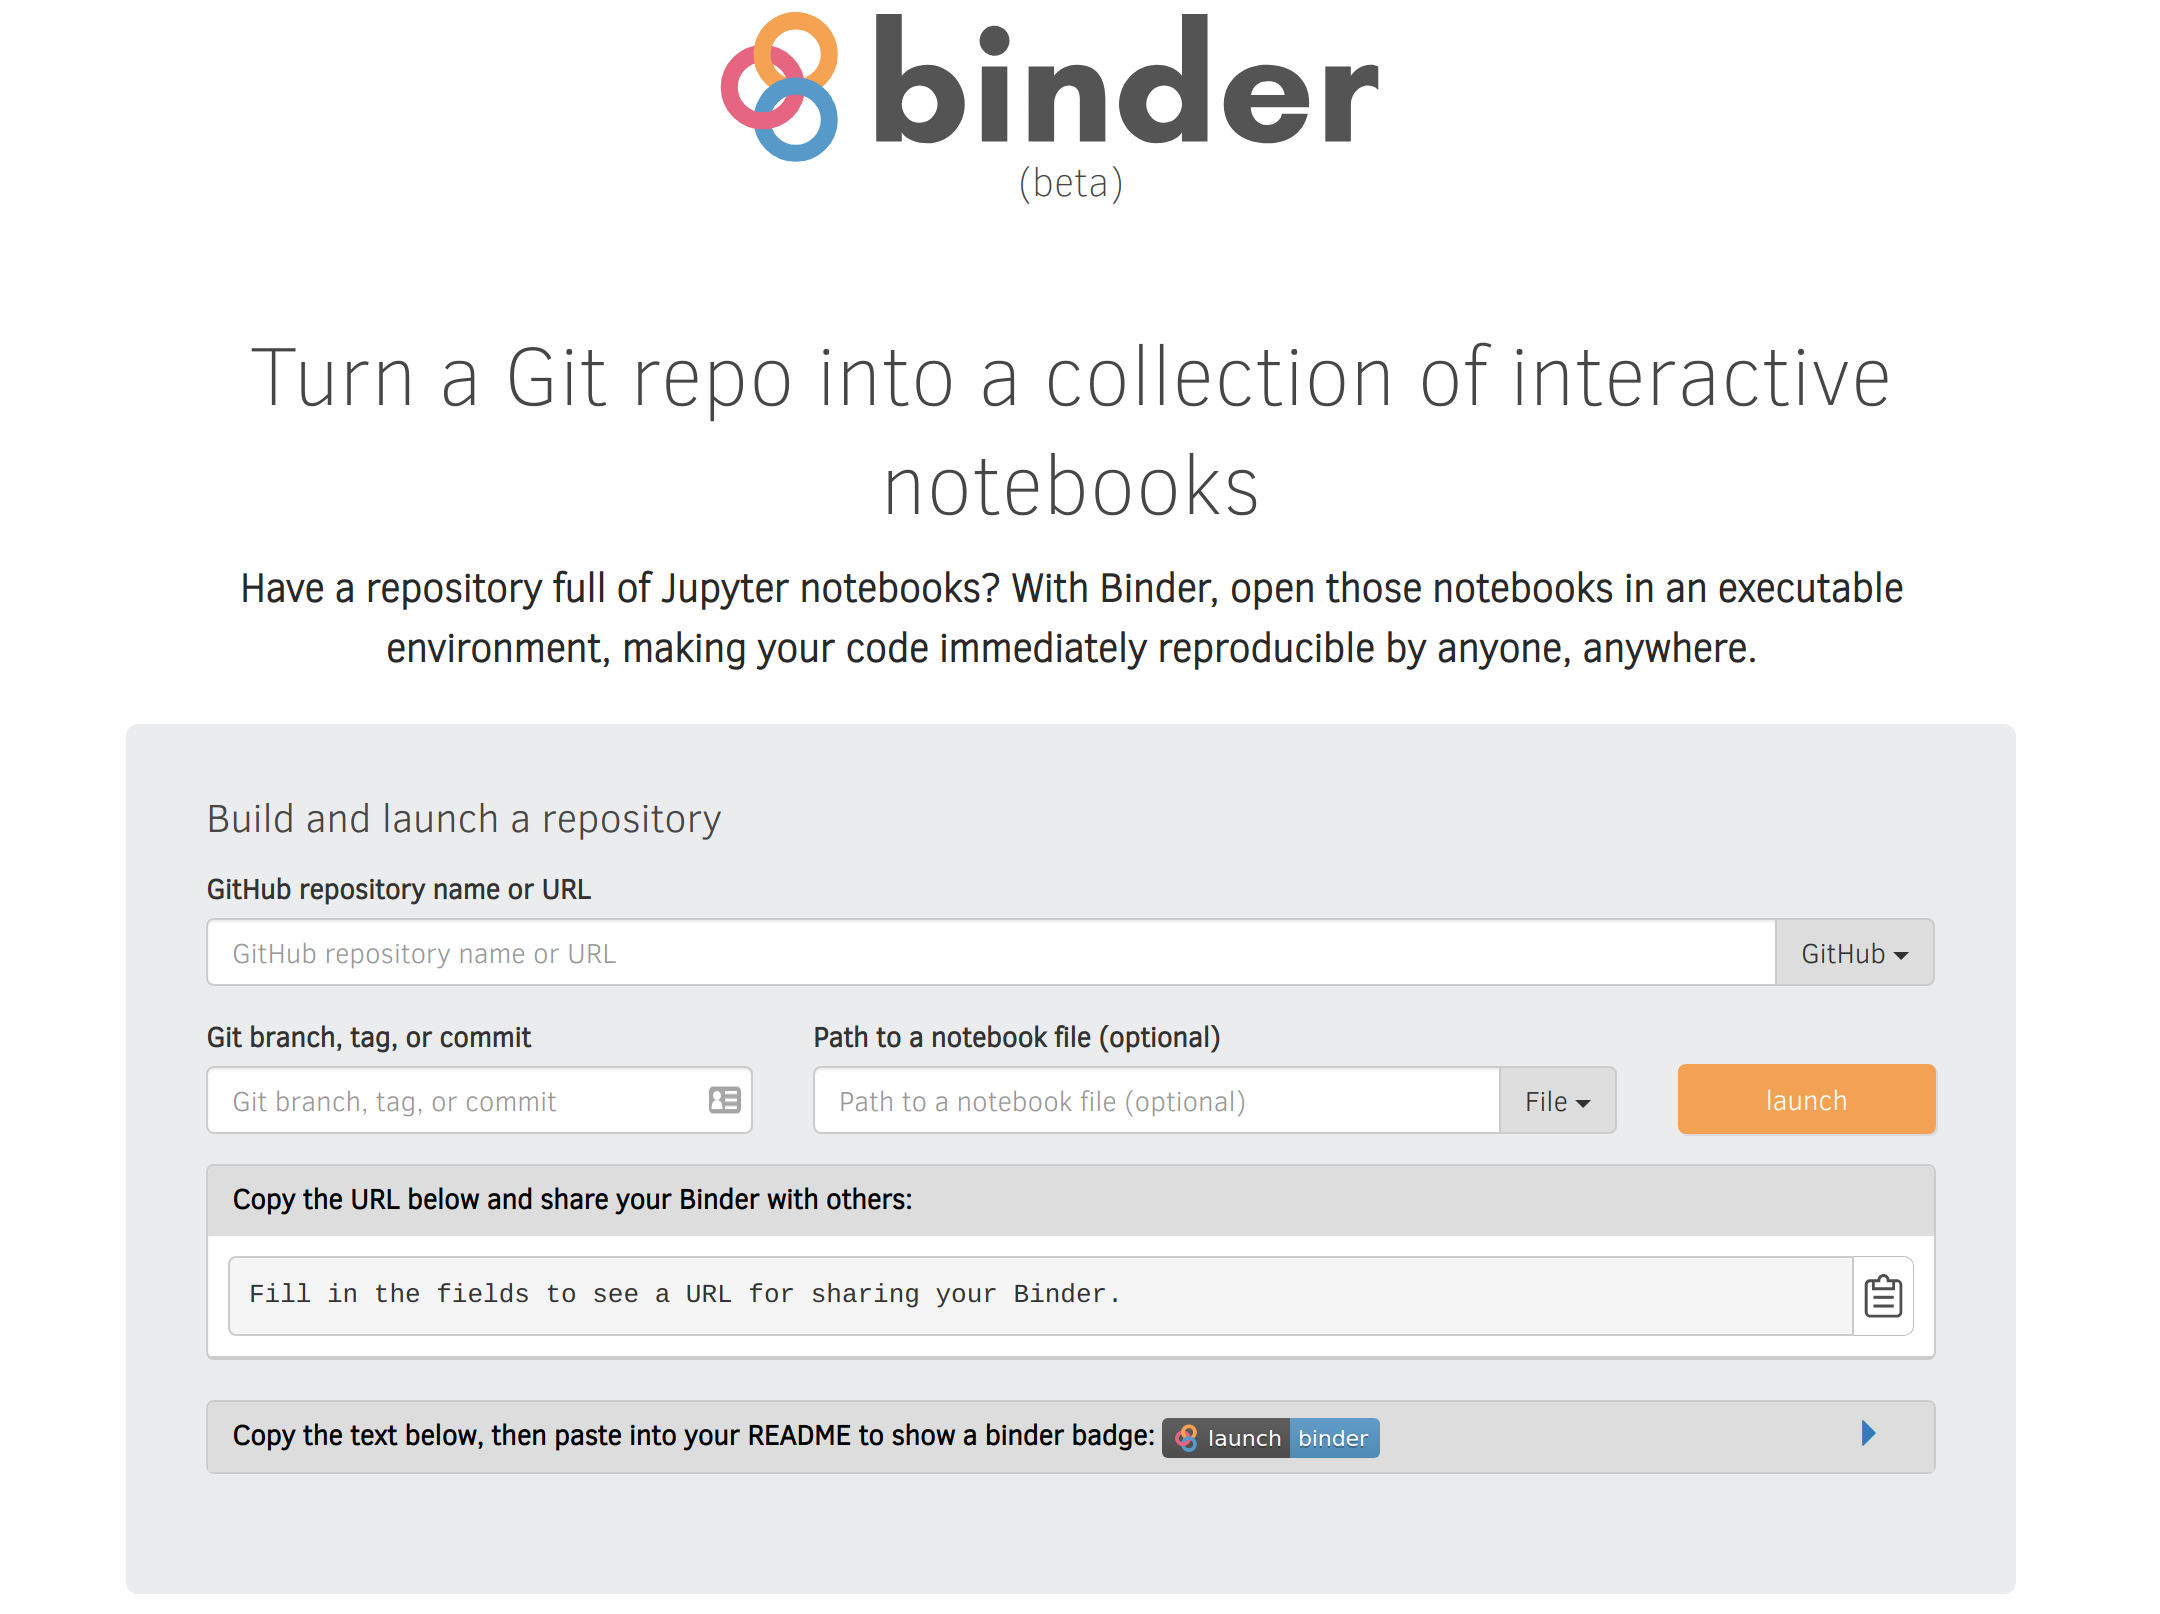
\includegraphics{binder-intro.png}
\caption{}
\end{figure}

    Si quieres compartir tus documentos Notebook con tus compañeros (o con
cualquier persona que no esté trabajando contigo en el Notebook),
utiliza Binder, ya que proporcionas un acceso sencillo y rápido
evitándoles tener que instalar todas tus dependencias, además de Jupyter
Notebook.

    \subsection{Google Colaboratory}\label{google-colaboratory}

    \href{https://colab.research.google.com/}{Google Colaboratory} es un
entorno Jupyter Notebook enfocado en la educación e investigación que te
permite realizar todo lo que podrías hacer con Jupyter Notebook en local
pero ejecutando tu código en sus servidores sin coste alguno. Además,
puedes almacenar los Notebook que crees y utilices en tu almacenamiento
Drive, para lo cual necesitarás una cuenta de Google (tu cuenta UCM
sirve, además, tendrás almacenamiento ilimitado con ella). Para utilizar
Google Colaboratory no es necesario tener instalado Jupyter Notebook,
además, funciona en cualquier sistema operativo. Simplemente accede a
https://colab.research.google.com en un navegador web moderno. Puedes
editar ficheros Notebook que hubieses creado y editado previamente en
local o con otras herramientas (cualquier fichero \texttt{.ipynb}),
además de editar ficheros Notebook almacenados en repositorios GitHub.
Al entrar por primera vez, verás únicamente una ventana similar a esta
que te introduce a la herramienta:

    \begin{figure}
\centering
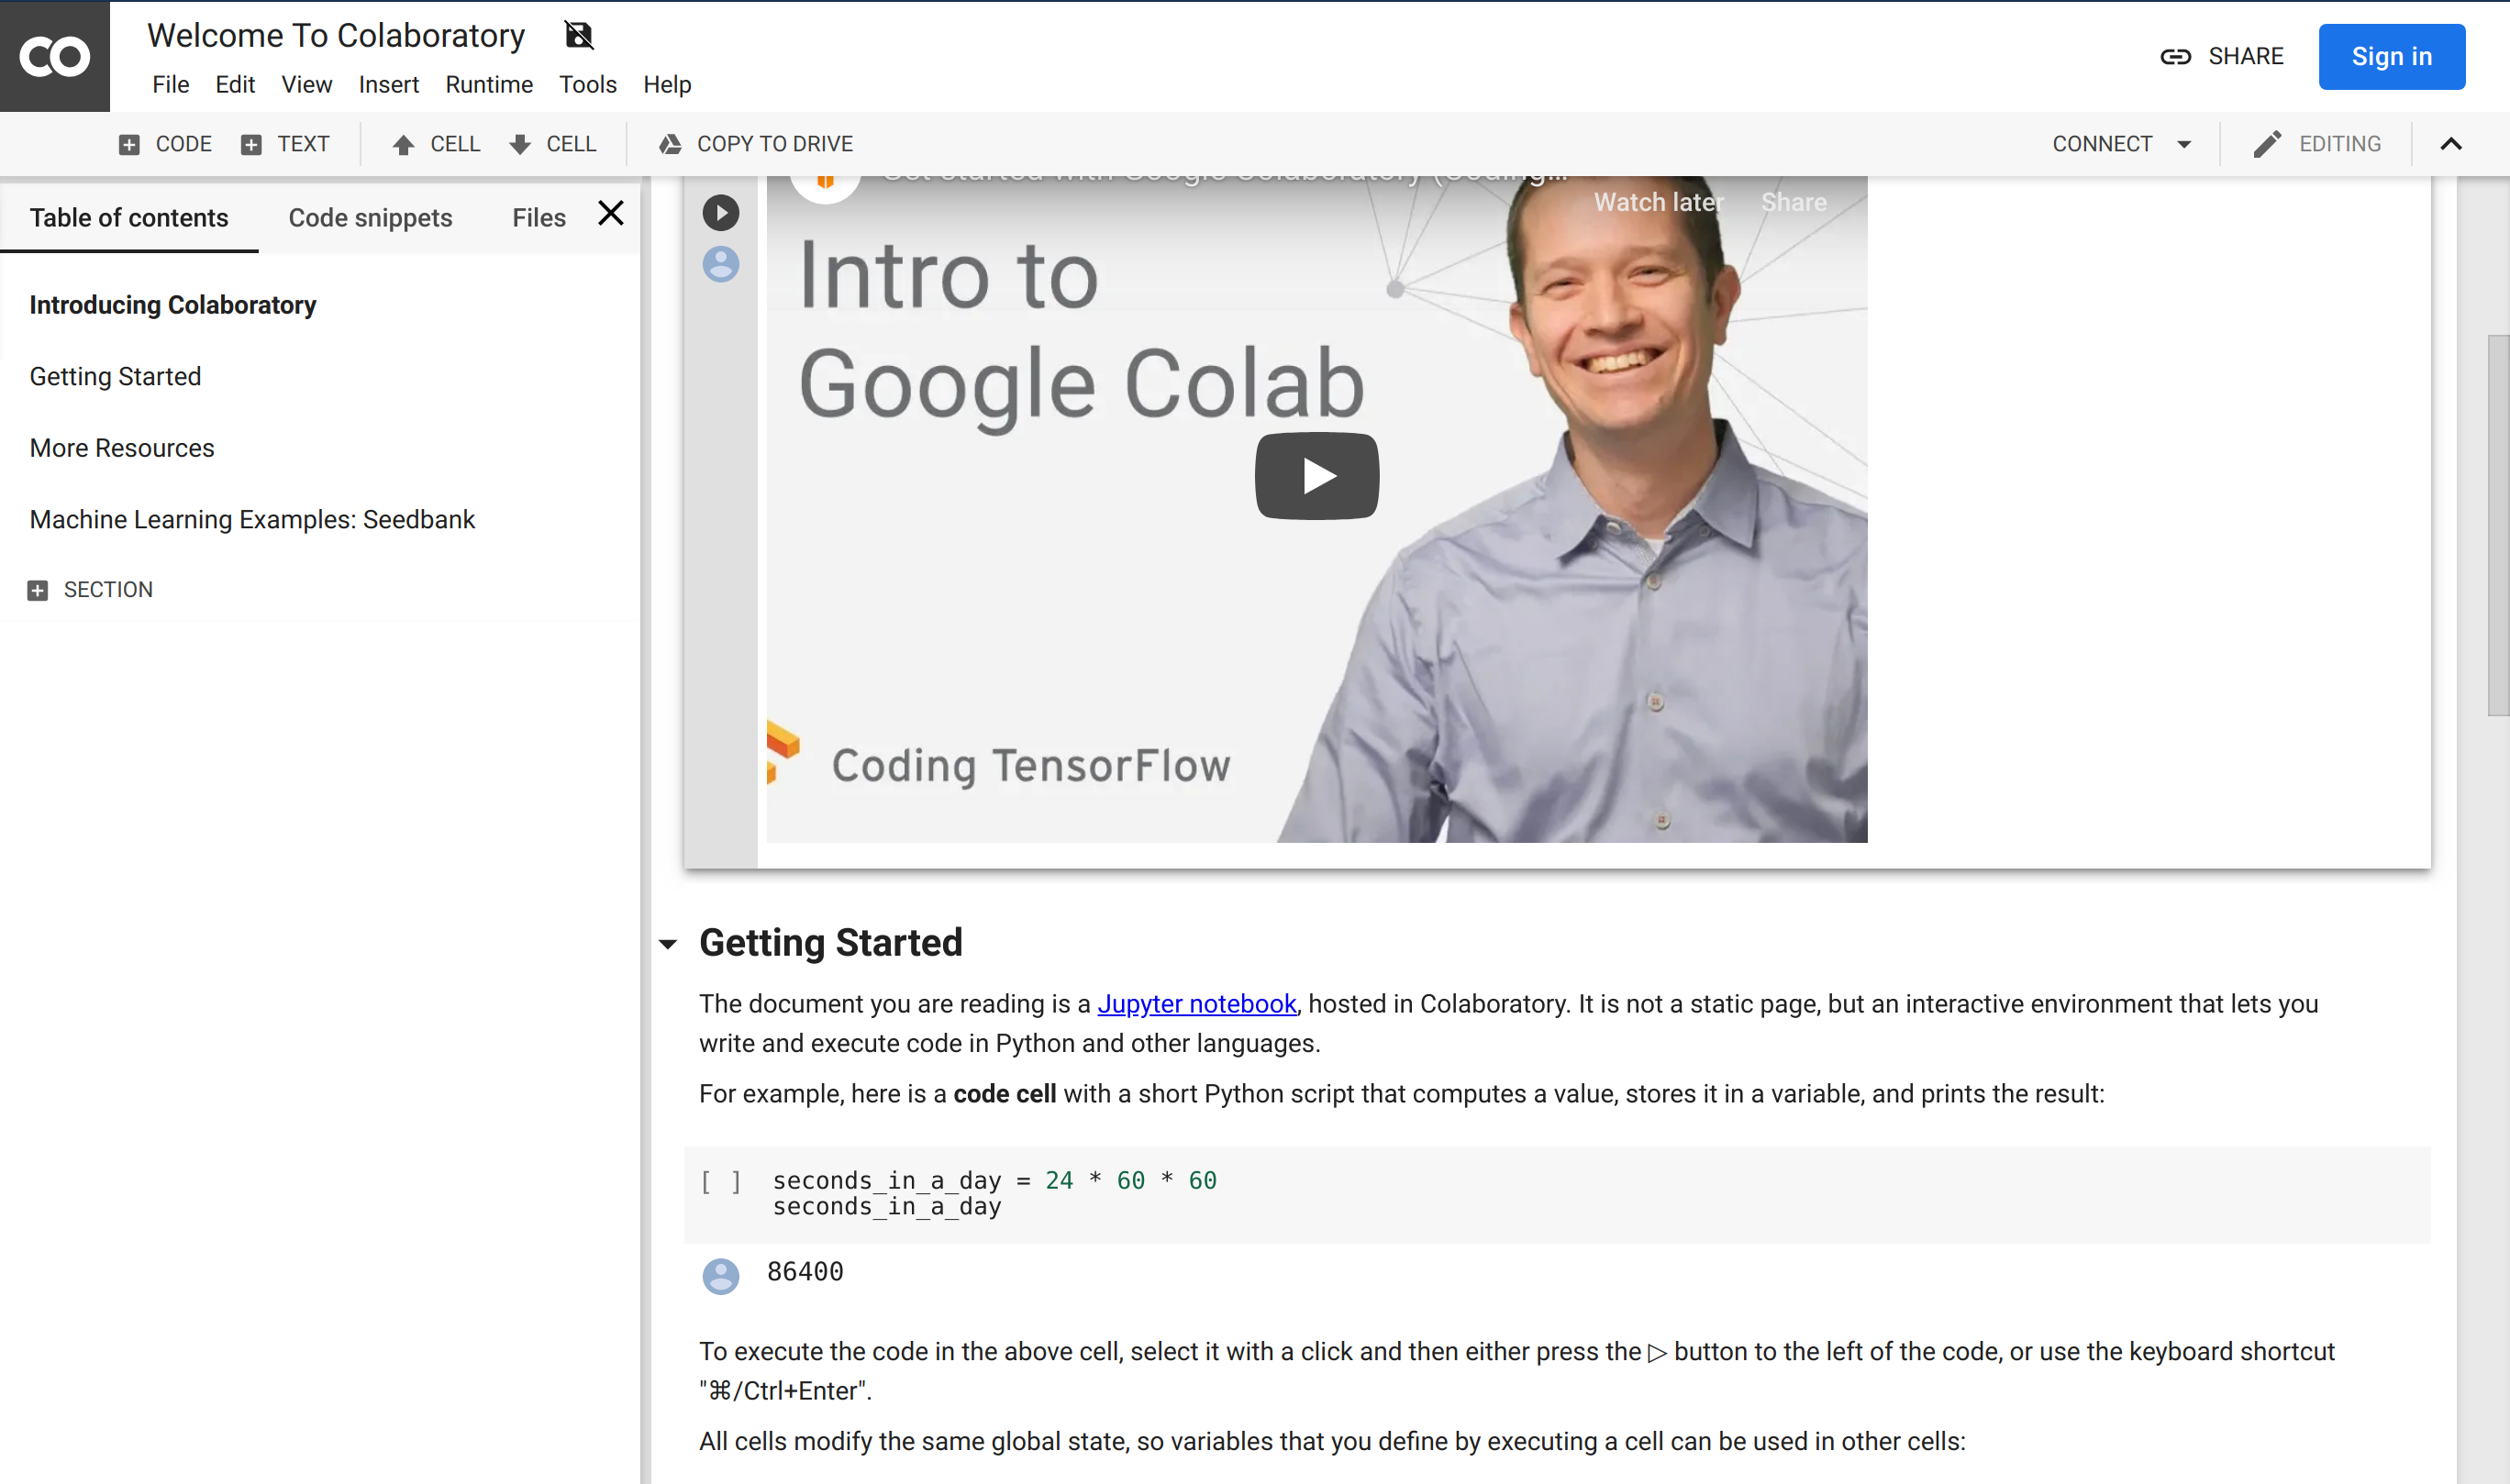
\includegraphics{gcolab-intro.png}
\caption{gcolab}
\end{figure}

    Una vez te hayas logueado, podrás guardar ficheros Notebook en tu unidad
Drive o abrir ficheros ya guardados previamente.

    \begin{figure}
\centering
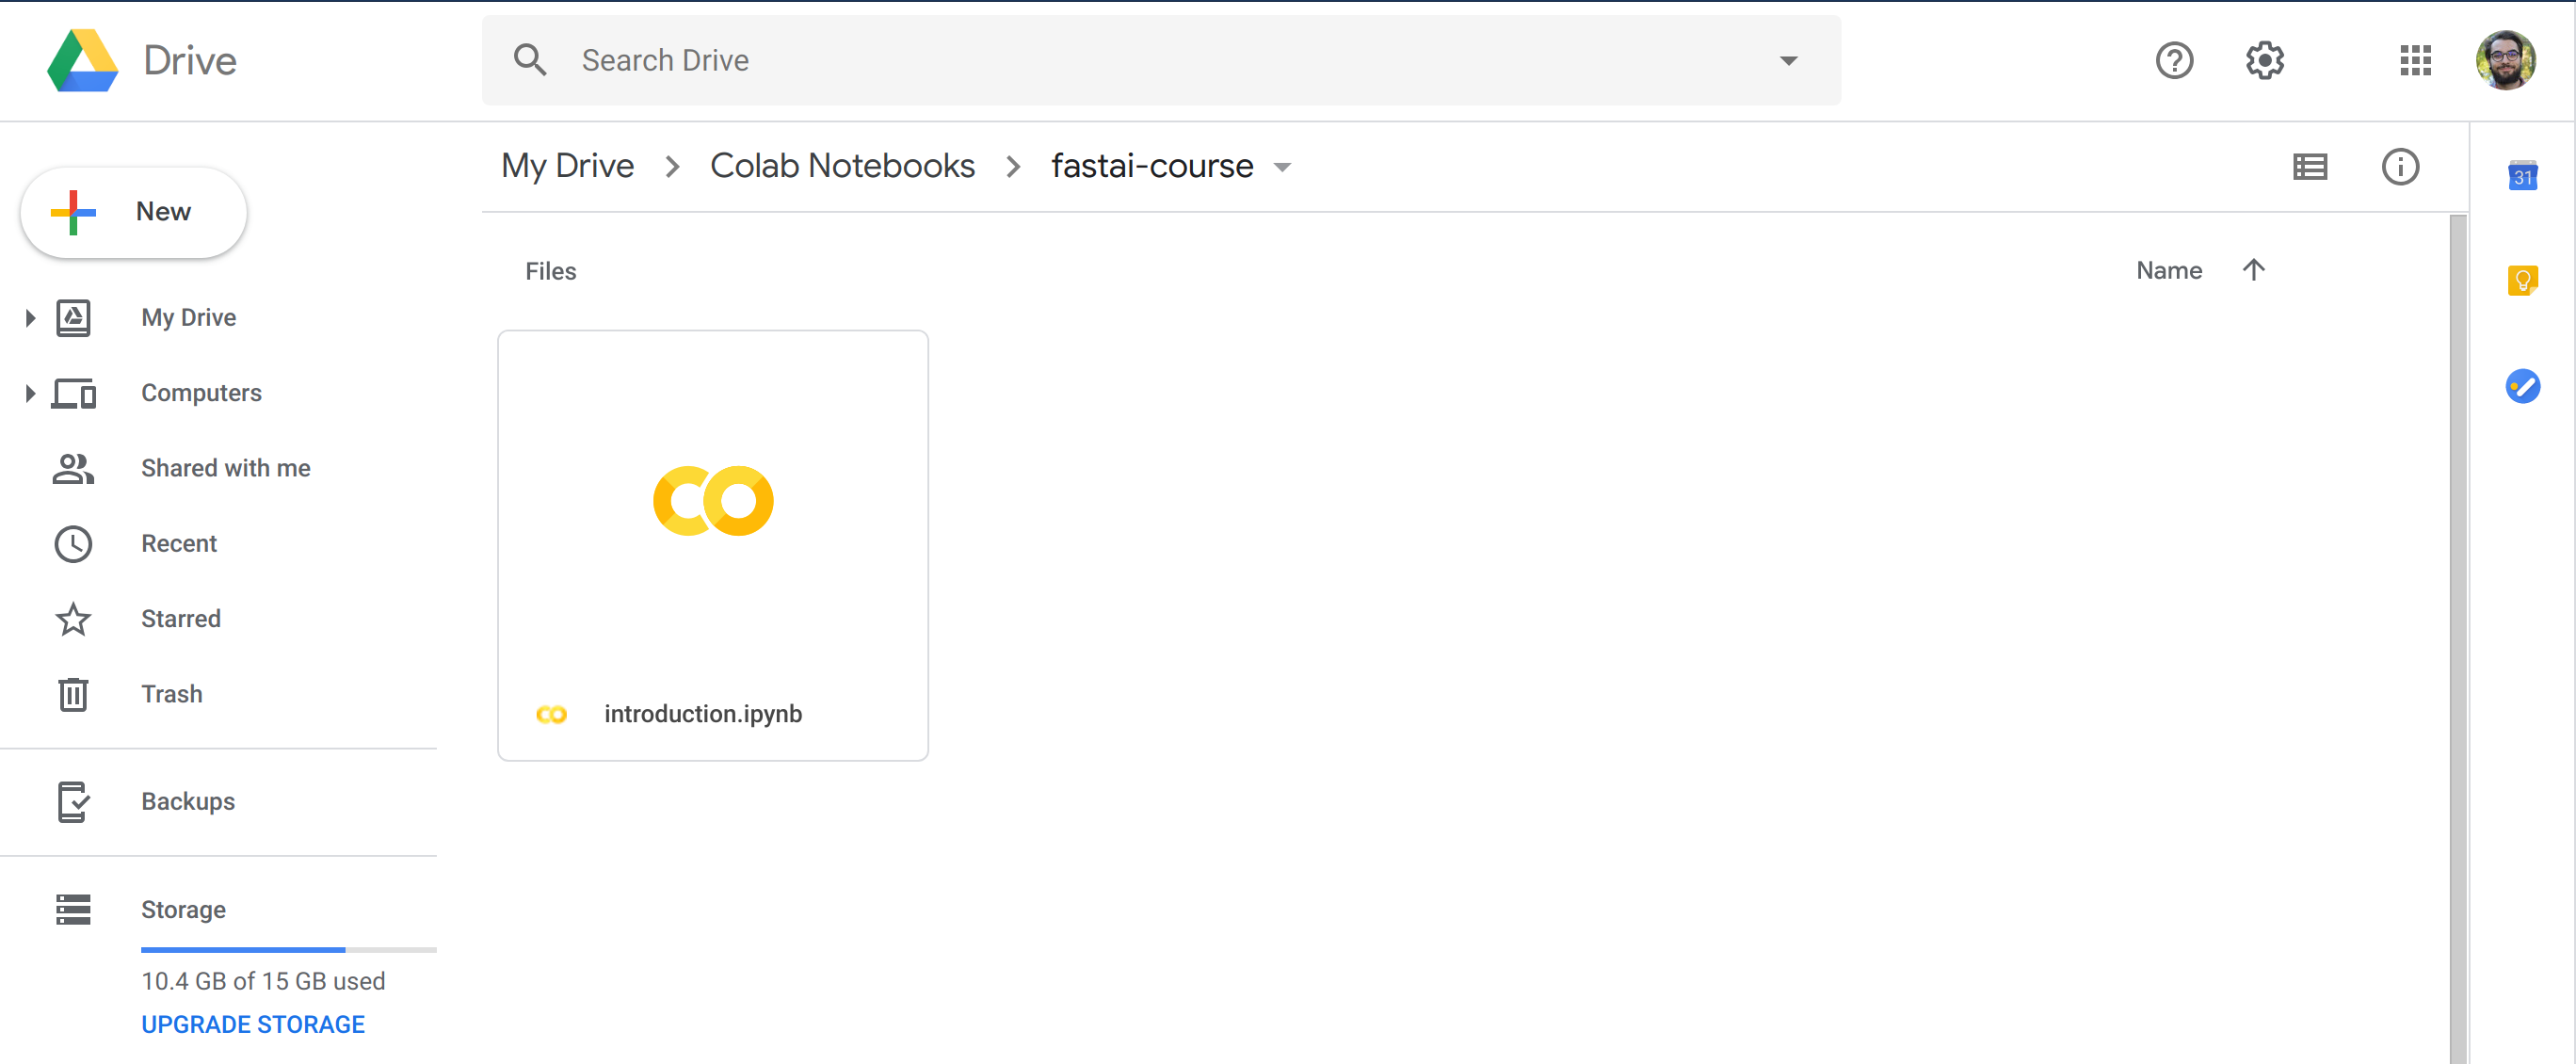
\includegraphics{gcolab-account.png}
\caption{gcolab account}
\end{figure}

    \subsubsection{¿Por qué es tan interesante Google
Colaboratory?}\label{por-quuxe9-es-tan-interesante-google-colaboratory}

    Google Colaboratory no ejecuta nada en tu ordenador, por lo tanto puedes
utilizar un ordenador con bajas prestaciones para realizar tus prácticas
de clase o preparar tus publicaciones sin preocuparte por la capacidad
de cómputo de tu ordenador. Además, puedes decidir que los servidores de
Google Colaboratory corran tus ejecuciones de celdas de código en GPU
(Tesla K80) o en TPU, en vez de la opción predeterminada, CPU.

    \begin{figure}
\centering
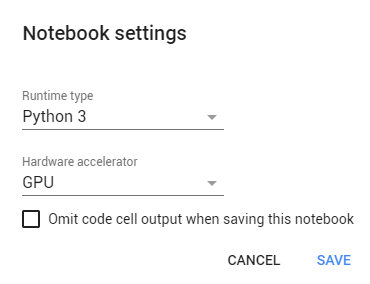
\includegraphics{gcolab-gpu.png}
\caption{}
\end{figure}

    \subsubsection{Algo malo tiene que tener Google
Colaboratory}\label{algo-malo-tiene-que-tener-google-colaboratory}

    El principal incoveniente de Google Colaboratory es que solo soporta
Python (3.6 y 2.7). Además algunas librerías, aunque sean populares, no
están instaladas en los sistemas en los que corre Google Colaboratory,
por lo cual necesitas ejecutar algunos pasos (una búsqueda en Google
debería ser suficiente para conocer qué pasos son) para instalar algunas
librerías. A pesar de ello, la gran mayoría de librerías de uso
científico en Machine Learning se encuentran instaladas y solo necesitas
importarlas.

    \begin{figure}
\centering
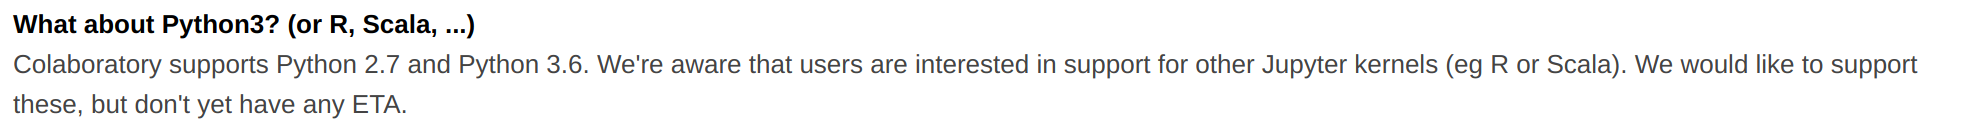
\includegraphics{gcolab-other-lang.png}
\caption{}
\end{figure}

    Si quieres trabajar en algún proyecto que requiera de gran capacidad de
computación (por ejemplo, entrenar modelos de Machine Learning) o tu
ordenador es muy antiguo, utiliza Google Colaboratory, ya que evitarás
preocuparte de muchos aspectos de correr Jupyter Notebook en local.

    \subsection{Ejemplos de Jupyter
Notebook}\label{ejemplos-de-jupyter-notebook}

    A continuación puedes visualizar algunos documentos Jupyter Notebook que
te pueden servir de ayuda en tu camino con la herramienta (todos los
enlaces te dirigen a documentos Notebook hosteados en Binder, por lo
cual podrás modificar cualquier celda y, por lo tanto, ver el
contenido): -
\href{https://mybinder.org/v2/gh/ehmatthes/intro_programming/master?filepath=notebooks/index.ipynb}{Introducción
a Python} -
\href{https://mybinder.org/v2/gh/albertopastormr/tic-tac-toe/master?filepath=\%2FTic-Tac-Toe_UCI.ipynb}{Tic-Tac-Toe
con Machine Learning} -
\href{https://hub.mybinder.org/user/jrjohansson-sci-python-lectures-5byenvty/notebooks/Lecture-4-Matplotlib.ipynb}{Introducción
a plotting con Matplotlib} -
\href{https://hub.mybinder.org/user/ipython-ipython-2f6w2d1v/notebooks/examples/IPython\%20Kernel/SymPy.ipynb}{SymPy}

También puedes encontrar ejemplos
\href{https://jupyter-notebook.readthedocs.io/en/stable/examples/Notebook/examples_index.html}{aquí}.

    \subsection{Siguientes pasos}\label{siguientes-pasos}

    Si llegados aquí te he convencido de utilizar Jupyter Notebook, te
recomiendo lo siguiente: - Si quieres utilizar Jupyter Notebook en local
para tener control máximo sobre tu documento, utiliza
\href{https://jupyter.readthedocs.io/en/latest/install.html}{este
tutorial} para realizar la instalación. - Si quieres utilizar Jupyter
Notebook pero no quieres instalarlo en tu ordenador, utiliza
\href{https://colab.research.google.com}{Google Colaboratory}, solo
varía su interfaz de usuario.


    % Add a bibliography block to the postdoc
    
    
    
    \end{document}
